% !Mode:: "TeX:UTF-8"

\section{各种测试}

\subsection{行数测试}
\clearpage
行数测试: 1\\
2\\
3\\
4\\
5\\
6\\
7\\
8\\
9\\
10\\
11\\
12\\
13\\
14\\
15\\
16\\
17\\
18\\
19\\
20\\
21\\
22\\
23\\
24\\
25\\
26\\
27\\
28\\
29\\
30\\
31\\
32\\
33\\
34\\
35\\
36\\
37\\
38\\
39\\


\begin{figure}[htbp]
    \centering
    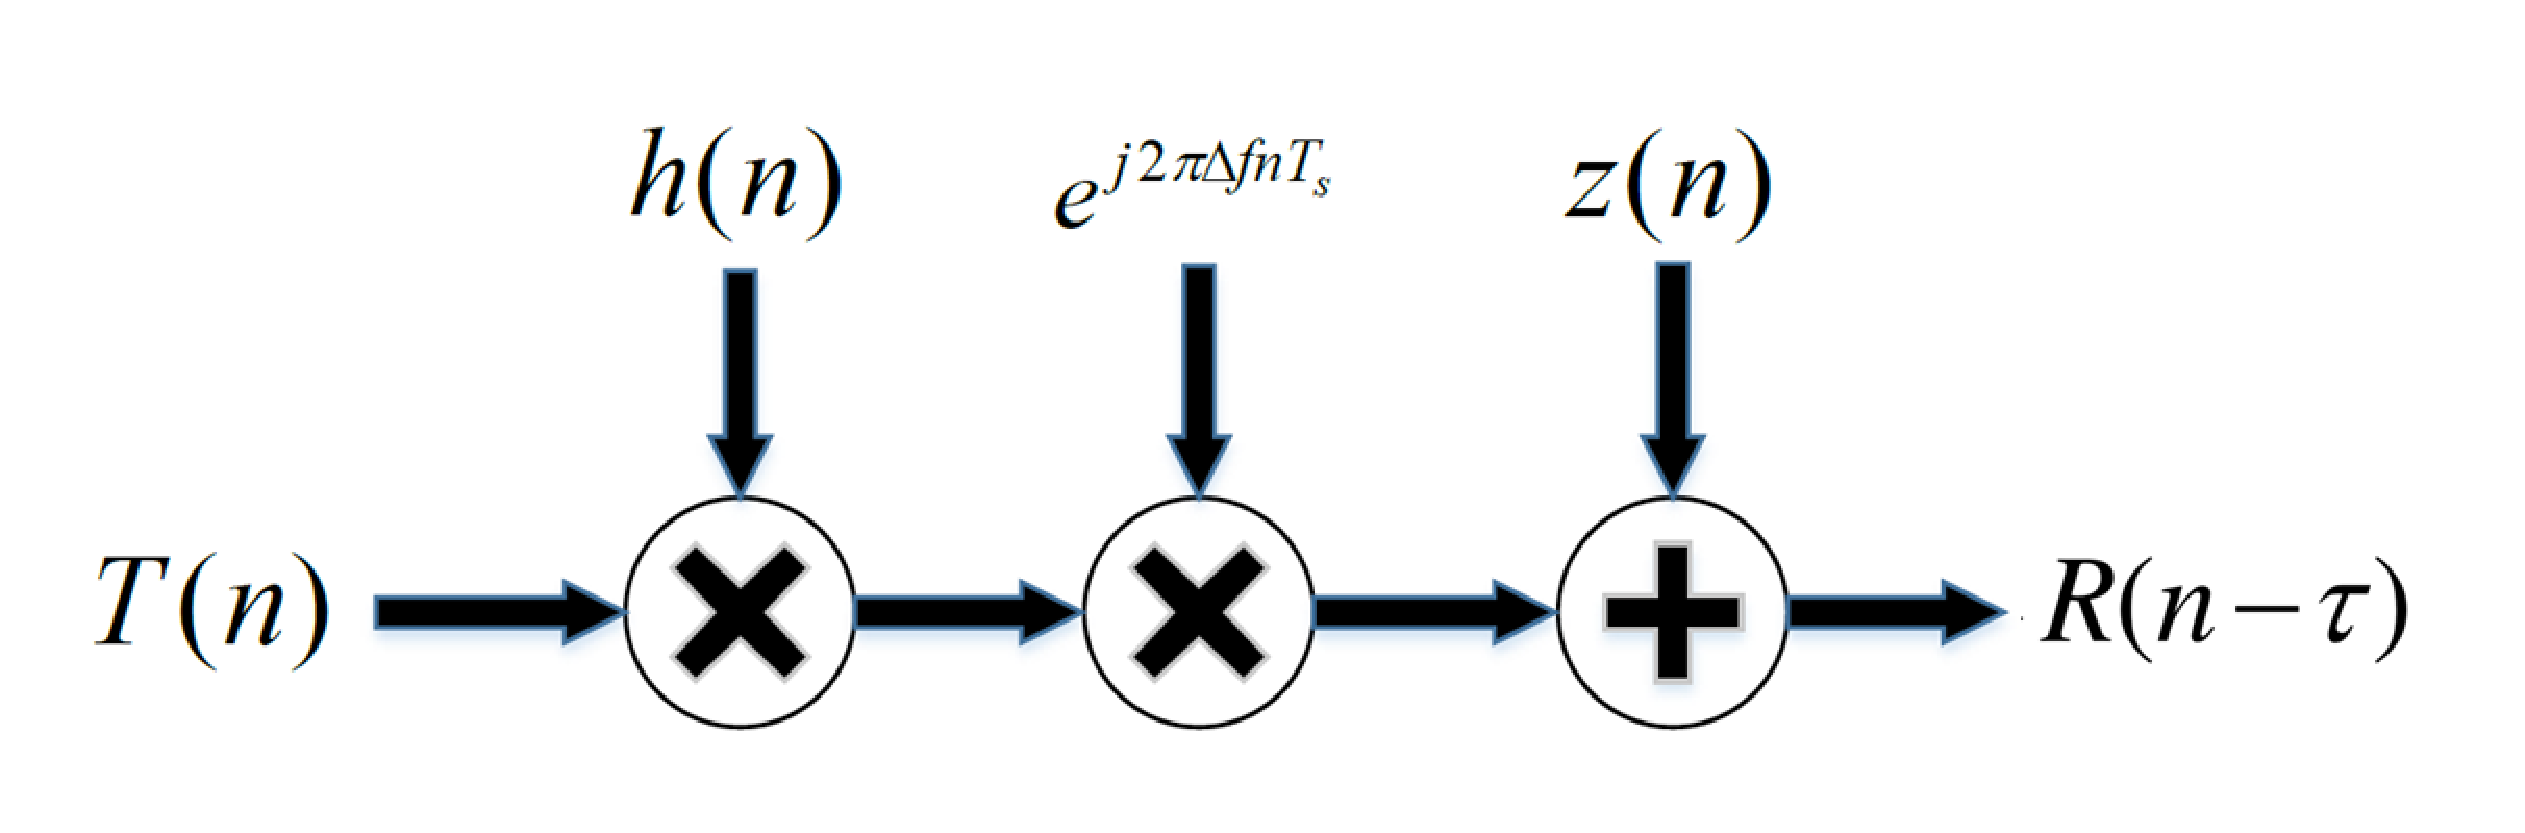
\includegraphics[width = 0.6\textwidth]{figure4_1.eps}
    \caption{引用测试:信道模型}\label{ref-test}
\end{figure}

autoref 引用测试 \autoref{ref-test}。


\begin{theorem}
    Let $f$ be a function whose derivative exists in every point, then $f$
    is a continuous function.
\end{theorem}

\begin{proof}
    To prove it by contradiction try and assume that the statement is false,
    proceed from there and at some point you will arrive to a contradiction.
\end{proof}

\begin{lemma}
    Given two line segments whose lengths are $a$ and $b$ respectively there
    is a real number $r$ such that $b=ra$.
\end{lemma}

多参考文献测试\cite{hui2015_177_179,lei2017,Mei2010The}。
